\documentclass[aspectratio=169,11pt]{beamer}
\usetheme{metropolis}
\usepackage{listings}
\usepackage{tikz}
\usetikzlibrary{arrows.meta,positioning,fit,backgrounds,calc,decorations.pathreplacing}
\usepackage{booktabs}
\usepackage{xcolor}

\definecolor{codegreen}{rgb}{0.2,0.6,0.2}
\definecolor{codegray}{rgb}{0.5,0.5,0.5}
\definecolor{codepurple}{rgb}{0.58,0,0.82}
\definecolor{tenantA}{RGB}{31,119,180}
\definecolor{tenantB}{RGB}{255,127,14}
\definecolor{tenantC}{RGB}{44,160,44}
\definecolor{shared}{RGB}{200,200,200}

\lstset{
  basicstyle=\ttfamily\scriptsize,
  keywordstyle=\color{codepurple}\bfseries,
  commentstyle=\color{codegray}\itshape,
  stringstyle=\color{codegreen},
  breaklines=true,
  columns=fullflexible,
  keepspaces=true,
}

\title{KV-Cache Residency Instrumentation in vLLM}
\subtitle{Per-Tenant Token-Seconds via Prometheus Counter}
\date{}

\begin{document}

% ============================================================
% SLIDE 1: Architecture
% ============================================================
\begin{frame}{Slide 1: Instrumentation Architecture}

\begin{columns}[T]
\begin{column}{0.42\textwidth}

\textbf{Incremental tracking}

\vspace{0.3em}
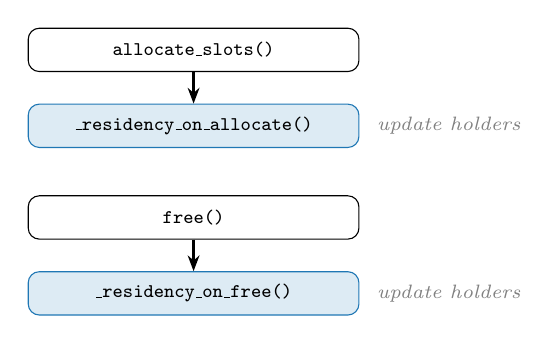
\begin{tikzpicture}[
    node distance=0.4cm,
    box/.style={draw, rounded corners, minimum width=4.2cm, minimum height=0.55cm, font=\scriptsize\ttfamily, align=center},
    hook/.style={draw, rounded corners, minimum width=4.2cm, minimum height=0.55cm, font=\scriptsize\ttfamily, align=center, fill=tenantA!15, draw=tenantA},
    arrow/.style={-{Stealth[length=2mm]}, thick},
]
    \node[box] (alloc) {allocate\_slots()};
    \node[hook, below=of alloc] (on_alloc) {\_residency\_on\_allocate()};
    \node[box, below=0.6cm of on_alloc] (free) {free()};
    \node[hook, below=of free] (on_free) {\_residency\_on\_free()};

    \draw[arrow] (alloc) -- (on_alloc);
    \draw[arrow] (free) -- (on_free);

    \node[right=0.1cm of on_alloc, font=\scriptsize\itshape, text=codegray] {update holders};
    \node[right=0.1cm of on_free, font=\scriptsize\itshape, text=codegray] {update holders};

\end{tikzpicture}

\vspace{0.4em}
{\scriptsize State lives on \texttt{KVCacheManager}. \\
Updated only when blocks change ownership.}

\end{column}
\begin{column}{0.56\textwidth}

\textbf{Per-step charging: O($N_{\text{tenants}}$)}

\vspace{0.3em}
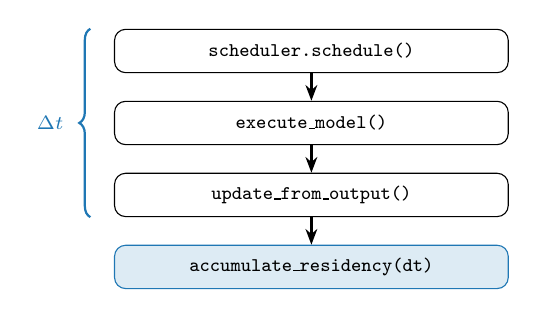
\begin{tikzpicture}[
    node distance=0.35cm,
    box/.style={draw, rounded corners, minimum width=5cm, minimum height=0.55cm, font=\scriptsize\ttfamily, align=center},
    charge/.style={draw, rounded corners, minimum width=5cm, minimum height=0.55cm, font=\scriptsize\ttfamily, align=center, fill=tenantA!15, draw=tenantA},
    arrow/.style={-{Stealth[length=2mm]}, thick},
]
    \node[box] (sched) {scheduler.schedule()};
    \node[box, below=of sched] (exec) {execute\_model()};
    \node[box, below=of exec] (update) {update\_from\_output()};
    \node[charge, below=of update] (resid) {accumulate\_residency(dt)};

    \draw[arrow] (sched) -- (exec);
    \draw[arrow] (exec) -- (update);
    \draw[arrow] (update) -- (resid);

    \draw[decorate, decoration={brace, amplitude=4pt, mirror}, thick, tenantA]
        ([xshift=-0.3cm]sched.north west) -- ([xshift=-0.3cm]update.south west)
        node[midway, left=6pt, font=\scriptsize, tenantA] {$\Delta t$};

\end{tikzpicture}

\vspace{0.2em}
{\scriptsize Reads \texttt{tenant\_resident\_tokens} dict. \\
No block iteration at step time.}

\end{column}
\end{columns}

\end{frame}

% ============================================================
% SLIDE 2: Pseudocode
% ============================================================
\begin{frame}[fragile]{Slide 2: Implementation Pseudocode}
\vspace{-0.7em}
\begin{columns}[T]
\begin{column}{0.47\textwidth}

\textbf{At allocation/free time (amortized):}
\vspace{-0.2em}
\begin{lstlisting}[language=Python, basicstyle=\ttfamily\tiny, morekeywords={self,for,in,if,not,elif,else,del}]
# On allocate block B for tenant T:
if B not in holders:
    holders[B] = {T: 1}
    tenant_tokens[T] += block_size
elif T not in holders[B]:
    k = len(holders[B])  # cross-tenant sharing
    for X in holders[B]:
        tenant_tokens[X] -= block_size/k
        tenant_tokens[X] += block_size/(k+1)
    holders[B][T] = 1
    tenant_tokens[T] += block_size / (k+1)
else:
    holders[B][T] += 1  # intra-tenant
# On free block B for tenant T:
holders[B][T] -= 1
if holders[B][T] == 0:
    k = len(holders[B])
    del holders[B][T]
    tenant_tokens[T] -= block_size / k
    for X in holders[B]:
        tenant_tokens[X] += block_size/(k-1)
                          - block_size/k
\end{lstlisting}

\end{column}
\begin{column}{0.51\textwidth}

\textbf{At step time --- O($N_{\text{tenants}}$):}
\vspace{-0.2em}
\begin{lstlisting}[language=Python, basicstyle=\ttfamily\tiny, morekeywords={self,for,in,if,not}]
def step():
    t0 = time.monotonic()
    schedule()            # allocates blocks
    execute_model()       # GPU forward pass
    update_from_output()  # frees completed reqs
    dt = time.monotonic() - t0

    # Charge all resident memory:
    for tenant, tokens in tenant_tokens.items():
        residency_counter.labels(
            tenant_id=tenant).inc(tokens * dt)
\end{lstlisting}

\vspace{0.2em}
\textbf{Conservation invariant:}
\vspace{-0.2em}
\begin{lstlisting}[language=Python, basicstyle=\ttfamily\tiny, morekeywords={self,for,in,if,not}]
# Always holds:
sum(tenant_tokens.values())
    == total_allocated_blocks * block_size
\end{lstlisting}

\vspace{0.1em}
{\scriptsize All GPU memory-time is fully accounted for. No over- or under-counting.}

\end{column}
\end{columns}

\end{frame}

% ============================================================
% SLIDE 3: Workload Design
% ============================================================
\begin{frame}{Slide 3: Workload Design}
\vspace{-0.2em}
\begin{columns}[T]
\begin{column}{0.48\textwidth}

\textbf{Experiment setup}

\vspace{0.2em}
{\scriptsize
\begin{itemize}\setlength{\itemsep}{0.2em}
    \item 1 model (e.g.\ Llama-3.1-8B), 1 GPU
    \item $N$ tenants ($\sim$3--5), each sends identical workload
    \item Same prompt length, output length, arrival rate
    \item Unique random prompts per request (no prefix cache hits)
    \item Prefix caching enabled but never triggers
\end{itemize}
}

\vspace{0.3em}
\textbf{What this tests}

\vspace{0.1em}
{\scriptsize
\begin{itemize}\setlength{\itemsep}{0.15em}
    \item Does the metric work end-to-end?
    \item Under symmetric load, is residency equal across tenants?
    \item Does the Prometheus counter accumulate correctly over time?
\end{itemize}
}

\end{column}
\begin{column}{0.50\textwidth}

\textbf{Configuration}

\vspace{0.2em}
{\scriptsize
\begin{tabular}{@{}ll@{}}
\toprule
\textbf{Parameter} & \textbf{Value} \\
\midrule
Tenants & 3 \\
Prompt length & 1024 words ($\approx$1032 tokens after chat template) \\
Max output tokens & 128 \\
Rate per tenant & 2 req/s (Poisson) \\
Duration & 5 min (300 reqs/tenant) \\
Model & Llama-3.1-8B \\
\bottomrule
\end{tabular}
}

\vspace{0.4em}
\textbf{Expected result}

\vspace{0.1em}
{\scriptsize
\begin{itemize}\setlength{\itemsep}{0.1em}
    \item Symmetric load $\to$ expect $\approx$ equal residency
    \item Any skew reveals scheduling unfairness (FCFS, batching, preemption)
    \item Conservation: $\sum$\texttt{rate(residency)} $=$ total KV blocks $\times$ \texttt{block\_size}
\end{itemize}
}

\end{column}
\end{columns}

\end{frame}

\end{document}
